%% AtrialSpectralBench --- compile-ready manuscript
%% Build:  cd docs/paper && latexmk -pdf manuscript.tex   (or: pdflatex manuscript.tex x2)
%% Self-contained: uses \thebibliography (no external .bib), figures in ./figures/.
%% All numbers trace to results/*.json; this is an in-silico computational study.
\documentclass[11pt]{article}

\usepackage[utf8]{inputenc}
\usepackage[T1]{fontenc}
\usepackage{lmodern}
\usepackage[a4paper,margin=1in]{geometry}
\usepackage{amsmath,amssymb,amsthm,mathtools}
\usepackage{graphicx}
\usepackage{booktabs}
\usepackage{array}
\usepackage{tabularx}
\usepackage{caption}
\usepackage{subcaption}
\usepackage{float}
\usepackage{enumitem}
\usepackage{xcolor}
\usepackage{microtype}
\usepackage{url}
\usepackage[colorlinks=true,linkcolor=black,citecolor=black,urlcolor=blue!55!black]{hyperref}

\graphicspath{{figures/}}

\newtheorem{theorem}{Theorem}
\newtheorem{lemma}{Lemma}
\theoremstyle{definition}
\newtheorem{definition}{Definition}

\newcommand{\lam}{\lambda}
\newcommand{\phii}{\varphi}
\newcommand{\rhoval}{\rho}
\newcommand{\SFI}{\mathrm{SFI}}
\newcommand{\dAUC}{\Delta\mathrm{AUC}}
% \code: monospace, with robust break opportunities after / and _ in long paths
\newcommand{\code}[1]{\texttt{#1}}
\emergencystretch=2em
% Tolerate imperceptible looseness (badness < 2500) around long verbatim paths/DOIs.
\hbadness=2500

\title{\textbf{AtrialSpectralBench}: a pre-registered test of a spectral
fragility biomarker for atrial reentry\\[4pt]
\large A feature-redundancy null, an estimator-validity boundary, and the
false positives naive methodology would have produced}

\author{Mounish Mavuduru\thanks{Independent, unaffiliated in-silico
computational-cardiology project. Correspondence and full source: see the
project repository.}}

\date{July 2026 (working preprint)}

\begin{document}
\maketitle

\begin{abstract}
\noindent
We ask whether a closed-form spectral graph biomarker predicts reentry
inducibility in atrial tissue beyond established fibrosis and connectivity
features. The biomarker is the \textbf{Spectral Fragility Index (SFI)}, the
Fiedler-value sensitivity $\partial\lam_2/\partial w_{ij}=(\phii_i-\phii_j)^2$
aggregated under a fibrosis-weighted conduction-uncoupling field. Pre-registered
before any labels were seen, the primary endpoint was $\dAUC\geq 0.05$ with a
DeLong paired $p<0.05$ on shape-family-held-out folds. \emph{The endpoint is not
met, but the strength of the negative differs by regime, and we separate them.} On up to $100{,}000$ synthetic excitable networks SFI adds no practically
meaningful predictive value (subspace $\dAUC\approx+0.003$; $\sim\!4{,}150$ cases
needed at $80\%$ power, resolvable only because $N$ is huge, and so
\emph{clinically undetectable} there). On two real cohorts ($182$ patients:
Roney $n=100$, UW/Boyle $n=82$) the combined gradient-boosting estimate is
$+0.012$ with a bootstrap interval $[-0.017,+0.044]$ that excludes the
threshold, so the real-anatomy result is a measured null rather than a
shortfall of power. An earlier version of this work reported $+0.051$ here and
called the real-cohort evidence inconclusive. That figure was an artefact of a
defect in one cohort's released substrate, which we found only afterwards; the
audit that found it, and the three controls that failed to explain everything
it left behind, are reported in full. Where the
null is clean, the mechanism is feature
redundancy: the exact per-region $\Delta\lam_2$ SFI, which has no first-order
approximation error, also adds nothing over the competitor set. A separate,
label-free result explains why the \emph{single-vector} SFI is also
ill-conditioned on real tissue. It is valid only while
$\rhoval=\lVert\Delta L\rVert/(\lam_3-\lam_2)=O(1)$, and real atria have
$\rhoval\approx 2422$ ($\sim\!10^3\times$ past the empirical
$\rhoval^\ast\approx 3$), so by Davis--Kahan the Fiedler vector is unstable. We do \emph{not} claim $\rhoval$ proves non-predictiveness; it bounds the
accuracy of the $\Delta\lam_2$ \emph{magnitude}, not the classification content
of a ranking feature. The spectral gap collapses as $N^{-1.05}$ on the real
atrial surface (the 2-manifold Weyl exponent), so $\rhoval$ grows lawfully with
resolution. One component partially survives: the Fiedler-gradient localizer
$\lvert\nabla\phii_2\rvert$ is a weak but real rank localizer (origin in the top
$\sim\!18\%$) that beats graph-centrality baselines and transfers across three
dynamical media, though it \emph{coincides with}, and does not beat, substrate
imaging, by a mechanism we make precise. Naive methodology (random CV,
$p$-value thresholds, no effect-size gate) would have reported SFI as working;
our pre-registered protocol rejects it. Our own convergence study surfaces a key
limitation: the inducibility labeller over-calls at the operating mesh
resolution and, on a completed six-tier study ($1500$--$48000$ nodes, $n=24$),
does not converge within the tested window. Our contribution is a carefully
bounded negative result: the mechanism behind it, a label-free criterion for the
estimator's validity, a characterization of how it scales, and a demonstration of
the false positives that standard methodology produces.
\end{abstract}

\noindent\textbf{Keywords:} algebraic connectivity; Fiedler value; spectral
graph theory; atrial fibrillation; reentry; biomarker; perturbation theory;
validity radius; pre-registration; negative result.

\medskip
\noindent\emph{This is a 100\% in-silico computational study. Ground-truth
labels are electrophysiology-simulator inducibility verdicts, never clinical
outcomes. All numbers trace to \code{results/*.json} and
\code{notebooks/lab\_notebook.md} in the project repository.}

\tableofcontents

%======================================================================
\section{Introduction}
%======================================================================
Algebraic connectivity $\lam_2$ (Fiedler 1973~\cite{fiedler1973}) governs the
stability of coupled excitable and oscillator networks (the
master-stability-function result~\cite{pecora1998} and the synchronizability
eigenratio $\lam_N/\lam_2$~\cite{barahona2002}), and has been used as a
real-time seizure detector~\cite{bomela2020}. The per-edge sensitivity
\begin{equation}
\frac{\partial\lam_2}{\partial w_{ij}}=(\phii_{2,i}-\phii_{2,j})^2
\label{eq:edge}
\end{equation}
is a classical identity underlying Fiedler-vector edge-editing
heuristics~\cite{ghosh2006}. It is therefore natural to hypothesize that
aggregating this sensitivity over a fibrosis-weighted perioperative uncoupling
field yields a per-region biomarker of atrial-fibrillation (AF) reentry
fragility. We test this hypothesis and \emph{pre-register the null}
(``SFI merely re-encodes fibrosis'') as an accepted, reportable outcome,
so that a negative result is a success of the protocol rather than a
file-drawer casualty.

The mathematics we use is classical; we claim no new theorem. Our contributions are
(i)~a leakage-controlled incremental test of SFI against real competitors and a
spatial null on real anatomy; (ii)~a validity criterion and a Weyl scaling law
that explain the failure and predict it for the whole class of spectral
fragility biomarkers; (iii)~a cross-medium transfer analysis isolating the one
component that generalizes; and (iv)~a falsification-protocol demonstration
showing that standard methodology would have manufactured exactly the false
positive this protocol catches.

In brief, a closed-form spectral
fragility index does \emph{not} add practically meaningful reentry-inducibility
prediction beyond existing features, either at synthetic scale or on $182$
patients of real anatomy, and the mechanism is feature redundancy. Independently, the
single-vector estimator is provably ill-conditioned on real tissue
($\rhoval\gg 1$). What we report is not a discovery but a carefully drawn
boundary: where a Fiedler-based estimator is numerically valid, why real tissue
lies far outside it, and how readily naive methodology mistakes redundant,
inconclusive signal for a working biomarker.

%======================================================================
\section{Theory: the Spectral Fragility Index}
\label{sec:theory}
%======================================================================
The core mathematics is classical numerical linear algebra; the
contribution is its \emph{use}. We state each result with its prior art
(Section~\ref{sec:credits}) and make the validity boundary explicit
(Section~\ref{sec:validity}).

\subsection{The weighted conduction graph}
Nodes are mesh vertices; edges are triangle edges; the edge weight $w_{ij}>0$
is a fibre-anisotropic conduction conductance attenuated by local fibrosis. The
combinatorial Laplacian is
\begin{equation}
L=D-W,\qquad D=\operatorname{diag}\Big(\textstyle\sum_j w_{ij}\Big).
\end{equation}
$L$ is symmetric positive-semidefinite with a single zero eigenvalue (the
constant vector) for a connected graph, with spectrum
$0=\lam_1<\lam_2\leq\lam_3\leq\cdots$ and eigenvectors $\phii_1,\phii_2,\dots$;
$\lam_2$ is the algebraic connectivity and $\phii_2$ the Fiedler vector.

\subsection{The closed-form fragility (first order)}
$L$ is a sum of rank-one edge terms, so
\begin{equation}
L=\sum_{(i,j)\in E} w_{ij}\,(e_i-e_j)(e_i-e_j)^{\!\top}
\;\Longrightarrow\;
\frac{\partial L}{\partial w_{ij}}=(e_i-e_j)(e_i-e_j)^{\!\top}.
\label{eq:dL}
\end{equation}
For a \emph{simple} eigenvalue $\lam$ with unit eigenvector $\phii$,
first-order (Hellmann--Feynman) perturbation theory gives
$\partial\lam/\partial w_{ij}=\phii^{\!\top}(\partial L/\partial w_{ij})\phii
=(\phii_i-\phii_j)^2$, which for the Fiedler pair is Eq.~\eqref{eq:edge}: a
non-negative per-edge \emph{fragility}. Reducing a conductance $w_{ij}$ by a
small $\Delta w_{ij}\geq 0$ (uncoupling) lowers $\lam_2$ by
$\Delta w_{ij}(\phii_{2,i}-\phii_{2,j})^2$ to first order.

The identity is verified in seven independent ways rather than merely asserted.
Computer algebra: sympy proves Eqs.~\eqref{eq:edge}--\eqref{eq:dL} symbolically,
and on a concrete $5$-node graph the finite-difference
$\partial\lam_2/\partial w_{ij}$ matches $(\phii_{2,i}-\phii_{2,j})^2$ to
$\lvert\text{err}\rvert\approx 2\times10^{-17}$ (mpmath, $40$ digits). Exactness:
the identity holds \emph{exactly} with rational weights (zero floating point);
an interval-arithmetic enclosure certifies the true $\lam_2$ to within
$\sim\!4\times10^{-40}$; and $\lam_2/\phii_2$ agree across scipy, networkx, and a
hand-rolled inverse iteration (spread $2.5\times10^{-15}$). The
algebraic core is kernel-checked in the Coq proof assistant over the
exact rationals, axiom-free (Appendix~\ref{app:formal}). The analytic
Hellmann--Feynman step (differentiability of a simple eigenvalue) is the cited
classical result~\cite{ghosh2006}, not re-proved here.

\subsection{Per-region aggregation: the SFI}
Model diffuse perioperative stress as a distribution of small, non-negative,
fibrosis-weighted fractional conductance reductions $\Delta w$ (mean
$\mathbb{E}[\Delta w_{ij}]=\mathrm{frac}_{ij}\,w_{ij}$, calibrated to literature
perioperative conduction-velocity slowing; $\Delta w\approx 0.36$, frozen in the
pre-registration). The per-region Spectral Fragility Index is the expected
$\lam_2$ drop contributed by region $R$:
\begin{equation}
\SFI(R)=\mathbb{E}[\Delta\lam_2\text{ from }R]
\approx\underbrace{\sum_{(i,j)\in R}\mathbb{E}[\Delta w_{ij}]\,(\phii_{2,i}-\phii_{2,j})^2}_{\text{first order}}
+\underbrace{\sum_{k\neq2}\frac{(\phii_k^{\!\top}\Delta L\,\phii_2)^2}{\lam_2-\lam_k}}_{\text{2nd-order resolvent}}
+O(\lVert\Delta L\rVert^3).
\label{eq:sfi}
\end{equation}
The second-order term is the source of the validity radius below. Near
eigenvalue degeneracy ($\lam_2\approx\lam_3$) the single $\phii_2$ is an
arbitrary rotation in the low invariant subspace, so we use a basis-independent
\emph{subspace (projector) SFI}: with $P=\sum_c\phii_c\phii_c^{\!\top}$ over the
clustered subspace, $s_{ij}^{\!\top}Ps_{ij}=\sum_c(\phii_{c,i}-\phii_{c,j})^2$
($s_{ij}=e_i-e_j$) is well-defined. For discrete edits (Maze lesion,
atriotomy) the expansion is abandoned and $\lam_2$ is recomputed \emph{exactly}
after the rank-one edit.

\subsection{The validity radius (the central caveat)}
\label{sec:validity}
The first-order form is trustworthy only while the perturbation is small
\emph{relative to the spectral gap} $\lam_3-\lam_2$. Two different tools bound
two different things (a common error is to use Weyl for both):
\begin{itemize}[nosep,leftmargin=1.4em]
\item Weyl's inequality bounds the \emph{eigenvalue} move:
      $\lvert\Delta\lam_2\rvert\leq\lVert\Delta L\rVert$.
\item Davis--Kahan / Bauer--Fike~\cite{daviskahan1970} bound the
      \emph{eigenvector} move, which scales like
      $\lVert\Delta L\rVert/(\lam_3-\lam_2)$. This, not Weyl, governs when
      $\phii_2$ (hence the single-vector SFI) degrades.
\end{itemize}
Define the \emph{validity radius}
\begin{equation}
\rhoval:=\frac{\lVert\Delta L\rVert}{\lam_3-\lam_2}.
\end{equation}
From second-order Rayleigh--Schr\"odinger theory the relative error of the
first-order $\Delta\lam_2$ prediction is $\Theta(\rhoval)$, and the Fiedler
vector rotates by $\sin\angle(\phii_2,\phii_2')\leq\sqrt{2}\,\rhoval$
(Davis--Kahan). Empirically the error is $1\%$ at $\rhoval=0.3$, crosses $10\%$
at $\rhoval^\ast\approx 3$, and reaches $92\%$ at $\rhoval=28$, with Weyl holding
throughout. On real excitable media the gap is tiny, so $\rhoval$ is
enormous: atrial-cohort median $\rhoval\approx 2422$, about $10^3\times$ past
$\rhoval^\ast$.

The criterion $\rhoval$ proves that the
\emph{single-vector} first-order SFI is a numerically \emph{invalid estimator of
$\Delta\lam_2$} on real tissue, and that $\phii_2$ is ill-conditioned
(Davis--Kahan), a label-free statement about the estimator. It does
\emph{not} prove SFI is non-predictive: $\rhoval$ bounds the accuracy of the
$\Delta\lam_2$ \emph{magnitude}, not the classification content of a monotone
ranking feature; indeed the \emph{exact} $\Delta\lam_2$ SFI (no $\rhoval$
limitation) is \emph{also} non-predictive (Section~\ref{sec:null}), so the
predictive null is separately due to feature redundancy. Two caveats:
(i)~$\rhoval$'s numerator carries the fibrosis-weighted $\Delta w$ field, so only
its denominator $\lam_3-\lam_2$ is truly label-free; (ii)~$\rhoval^\ast\approx3$
is calibrated on a $16$-node path graph with a problem-dependent constant, so
``$10^3\times$ past $\rhoval^\ast$'' is order-of-magnitude, not exact.

\subsection{Prior art (this is not new mathematics)}
\label{sec:credits}
The identity~\eqref{eq:edge} is Ghosh \& Boyd (2006)~\cite{ghosh2006}; algebraic
connectivity is Fiedler (1973)~\cite{fiedler1973}; $\lam_2$ governing coupled
excitable/oscillator stability is Pecora \& Carroll
(1998)~\cite{pecora1998} with the eigenratio of Barahona \& Pecora
(2002)~\cite{barahona2002}; Weyl's law, Davis--Kahan, and second-order
perturbation theory are classical (1970s and earlier). No result in
Section~\ref{sec:theory} is a new theorem, and none is presented as one. The
contribution is recognizing that $\rhoval$ is the right \emph{a priori}
validity screen for a spectral fragility biomarker, measuring its violation on
real tissue, and using it to \emph{mechanistically explain} a negative result.

%======================================================================
\section{Methods}
\label{sec:methods}
%======================================================================
Full detail is in the pre-registration (\code{docs/\allowbreak PRE\_REGISTRATION.md}) and
theory note (\code{docs/\allowbreak SFI\_THEORY.md}); the endpoints, cross-validation scheme,
baseline set, and accepted null were frozen before any labels were inspected.

\paragraph{Substrate.} Real left-atrial surfaces are loaded into weighted
conduction graphs from two public cohorts: the Roney LA virtual cohort (Zenodo
5801337~\cite{roney2022}) and the UW/Boyle LGE-MRI cohort (Dryad
\code{10.5061/dryad.kkwh70sg0}, $82$ distinct AF patients~\cite{uwboyle2025}).
Each mesh carries universal atrial coordinates, an image-intensity-ratio (IIR)
fibrosis proxy mapped to a fibrosis field by the Khurram healthy-to-scar
ramp~\cite{khurram2014}, and fibre fields. Meshes are coarsened to
$\sim\!2000$-node graphs by field-preserving vertex clustering.

\paragraph{Labels.} Ground truth is a monodomain Mitchell--Schaeffer
reaction--diffusion inducibility verdict~\cite{mitchell2003} (self-sustained
reentry $\geq 650$~ms after burst pacing at cycle length $150$~ms from random
sites), run on each real anatomy with an anisotropic conductance-weighted
cotangent Laplacian and implicit time stepping. Reentry here is governed by
wavelength (CV$\times$ERP), source--sink mismatch, and unidirectional block,
\emph{never} by $\lam_2$, so a predictive SFI$\to$label link is not circular.
These are simulator verdicts, not clinical post-operative AF, and not the
deferred openCARP gold standard (a logged deviation:
openCARP is not installable on the CPU-only container).

\paragraph{The SFI feature and its competitors.} Per-region SFI is computed as
in Eq.~\eqref{eq:sfi} (first-order, subspace, and exact-recompute variants). It
is evaluated strictly as an add-on/ablation against a non-trivial competitor set
that it must beat: fibrosis burden, fibrosis spatial entropy, fibrosis patch
size, deterministic global min-cut (Stoer--Wagner), percolation threshold, and
$\lam_2$-alone (isolating what the \emph{SFI construction} adds over the bare
algebraic connectivity).

\paragraph{Evaluation protocol (the guards).} Pre-registered: shape-family
\code{GroupKFold} (each patient is its own group, so cross-validation is
patient-held-out; grouped \emph{and} naive AUC both reported so leakage is
visible), the DeLong paired test~\cite{delong1988} in its fast midrank
form~\cite{sunxu2014}, $\geq 10^4$ stratified bootstrap resamples, a
rotational/torus-shift spatial null for localization, tie-robust permutation
nulls, and a keep/delete rule deciding each sub-claim by \emph{measured}
correlation. Effect sizes are gated, not just $p$-values. The primary endpoint
requires \emph{both} grouped $\dAUC\geq 0.05$ \emph{and} DeLong $p<0.05$.

\paragraph{Transfer media.} The identical calculus is applied to
FitzHugh--Nagumo (FHN) excitable networks and Kuramoto phase-oscillator networks
(a different dynamical class), where $\lam_2$ governs synchronizability, to
separate what is a property of the mathematics from an accident of one dataset.

%======================================================================
\section{Results}
\label{sec:results}
%======================================================================

\subsection{The predictive null (primary endpoint not met), across cohorts and scale}
\label{sec:null}

\begin{table}[H]
\centering
\caption{Incremental predictive value of SFI over the full competitor set.
$\dAUC$ is grouped (leakage-controlled); logistic regression (lr) /
gradient-boosted trees (gbt). The endpoint (grouped $\dAUC\geq0.05$ \emph{and}
DeLong $p<0.05$) is met in no regime, and every interval on real anatomy
contains zero. The UW rows rest on eight positives and are uninformative rather
than null; note in particular that their base AUCs differ sharply between the
competitor and fibrosis-only baselines, which is what inflates the latter's
apparent increment (Section~\ref{sec:null}).}
\label{tab:null}
ootnotesize
\begin{tabularx}{\linewidth}{@{}l r l r X@{}}
\toprule
cohort / medium & events/$N$ & model & base AUC & SFI $\dAUC$ (95\% CI); $p$ \\
\midrule
Roney (real)      & 34/100 & lr  & $0.870$ & $-0.021$ $[-0.075,+0.033]$; $0.44$ \\
                  &        & gbt & $0.856$ & $+0.009$ $[-0.029,+0.046]$; $0.63$ \\
UW/Boyle (real)   & 8/82   & lr  & $0.834$ & $+0.000$ $[-0.073,+0.081]$; $1.00$ \\
                  &        & gbt & $0.748$ & $+0.035$ $[-0.095,+0.203]$; $0.67$ \\
Combined real     & 42/182 & lr  & $0.884$ & $-0.007$ $[-0.042,+0.029]$; $0.70$ \\
                  &        & gbt & $0.851$ & $+0.012$ $[-0.017,+0.044]$; $0.45$ \\
\midrule
FHN networks      & \multicolumn{3}{l}{$2{,}000$ networks} & $\leq +0.003$; $p\geq0.12$ \\
FHN networks      & \multicolumn{3}{l}{up to $100{,}000$}  & subspace $+0.0028$; $p<10^{-4}$ at $N\geq10^4$ \\
Kuramoto networks & \multicolumn{3}{l}{$500$ networks}     & $\leq +0.0036$; $p\geq0.38$ \\
\bottomrule
\end{tabularx}
\end{table}

\begin{figure}[H]
\centering
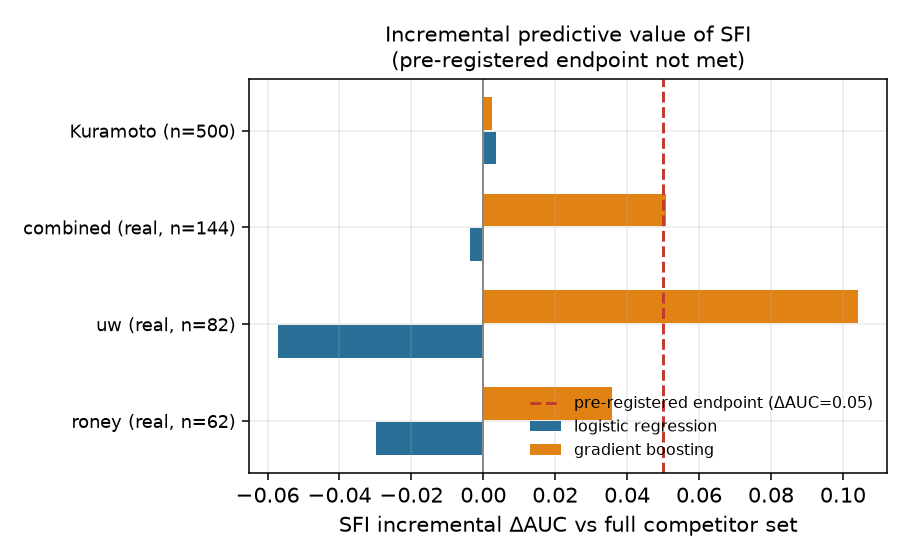
\includegraphics[width=0.86\linewidth]{fig_predictive_null.png}
\caption{The predictive null. Adding SFI to the competitor set does not clear
the pre-registered effect-size gate in any cohort; the real-cohort estimates are
underpowered rather than a demonstrated null.}
\label{fig:null}
\end{figure}

The negative is not uniform, and we separate the regimes. On the
\emph{synthetic} cohorts (up to $100{,}000$ networks) the null is clean: the
effect converges to $\dAUC\approx+0.003$, statistically resolvable only because
$N$ is enormous. On the \emph{real} cohorts it is underpowered and inconclusive.
The combined gradient-boosting point estimate is $+0.012$ (DeLong $p=0.449$,
bootstrap CI $[-0.017,+0.044]$), roughly a quarter of the pre-registered
$0.05$ threshold and with an interval that excludes it. An earlier version of
this analysis reported $+0.051$ here and had to argue that the endpoint was
missed only on significance. That estimate was an artefact of the sealed UW
substrate: correcting it drops the figure to $+0.036$ at the original cohort
size and to $+0.012$ once the Roney arm is extended to all $100$ released
meshes. With $42$ inducible of $182$ this is the largest real-anatomy arm in
the study, and the null here is a measurement rather than a shortfall.

The UW cohort remains the weak arm, though not for the reason we previously
gave. On eight positives its intervals are wide, the competitor comparison
spanning $[-0.095,+0.203]$ under gradient boosting, so it is an underpowered
external check of the \emph{labeller} rather than of SFI. We had also described
its competitor baseline as close to chance, and that was simply wrong: the
measured competitor base AUC is $0.834$ under logistic regression and $0.748$
under gradient boosting. Only the \emph{fibrosis-only} baseline approaches
chance, at $0.562$, and it is that near-chance baseline which manufactures the
cohort's largest apparent effect, $\dAUC=+0.217$ with $p=0.121$ and an interval
$[-0.030,+0.485]$ that spans half the available range. A large ratio over a
baseline that predicts almost nothing, on eight events, is not a signal.

The clean null comes from feature redundancy, not the validity radius. The
\emph{exact} per-region $\Delta\lam_2$ SFI, which carries no first-order
approximation error and is immune to the $\rhoval$ argument, also adds nothing
over the competitor set. The mechanism of the null is that SFI's information is
already present in standard connectivity features ($\lam_2$-alone, min-cut,
percolation), a label-dependent finding, separate from $\rhoval$.

\paragraph{Secondary endpoint (pre-specified), and its withdrawal.} An earlier
version of this analysis reported that SFI beat a
\emph{fibrosis-heterogeneity-only} baseline on the combined real cohort (GBT
$\dAUC=+0.103$, $p=0.009$) and read that as evidence SFI is not merely
re-encoded fibrosis but carries connectivity information beyond the substrate.
That result does not survive, and we withdraw both it and the claim it
supported. Two changes separate the old number from the new one, and they do
not contribute equally. Correcting the UW substrate while holding the cohort at
its original $144$ subjects leaves the estimate largely intact ($+0.093$,
$p=0.013$), so this was not principally a substrate artefact. Extending the
Roney arm from $62$ to the full $100$ released meshes is what collapses it, to
$\dAUC=+0.017$ ($p=0.452$). An effect that disappears when $38$ further real
subjects are added was a small-sample fluctuation, and it was one of
$\sim\!30$ DeLong comparisons besides. On the full cohort no comparison,
primary or secondary, shows SFI adding information beyond either baseline.

The discarded estimate is worth one more sentence, because its failure mode is
instructive. Under the sealed substrate the UW arm alone returned
$\dAUC=+0.340$ ($p=0.026$) on six positives, a value no one should have
believed and which we did not flag at the time; it is that arm which carried
the combined figure. A large point estimate resting on six events is a warning,
not a finding.

\paragraph{Power analysis.} In the synthetic cohort the subspace effect
($+0.0028$) needs $\sim\!4{,}150$ cases for $80\%$ power and the single-vector
effect ($+0.0007$) $\sim\!23{,}000$, clinically undetectable \emph{there}. We do
\emph{not} transport ``clinically undetectable'' to the real cohorts, whose
$+0.036$--$0.051$ estimates are compatible with a detectable effect we are simply
underpowered to confirm.

\subsection{Region definition and the patient-level reduction}
\label{sec:regions}

The per-region SFI of Eq.~(2) is stated over a region $R$, and until now we had
left $R$ implicit. Since the partition and the reduction that follows it are
what actually produce the feature block whose incremental $\dAUC$ is the primary
endpoint, we give both explicitly.

\paragraph{Partition.} Regions are a $3\times3$ grid over the universal atrial
coordinates. With $(\alpha,\beta)\in[0,1]^2$ per vertex, a vertex is assigned
$r=3\lfloor 3\beta\rfloor+\lfloor 3\alpha\rfloor \in\{0,\dots,8\}$, so every mesh
carries exactly nine regions regardless of its vertex count. An \emph{edge} is
assigned region $r$ only when both endpoints carry $r$; edges straddling two
regions go to a tenth bucket, $r=-1$, which is retained rather than discarded so
that the per-edge sensitivities sum to the global total. The rule is shared by
the closed-form and Monte-Carlo estimators so their region keys coincide.

This is where the two cohorts differ in kind and not only in degree. The Roney
meshes carry anatomically registered universal atrial coordinates, so their nine
regions are anatomical. The UW release ships none, so we substitute the top two
principal axes of the surface coordinates, min-max normalised. That surrogate is
a smooth two-dimensional chart adequate for binning, but it is not registered to
anatomy, and any region-level or localization claim on the UW cohort is
correspondingly weaker. The substitution is recorded in the mesh metadata rather
than left to the reader to infer.

\paragraph{Reduction to the patient.} The classification target is one binary
verdict per patient, so the nine per-region values must be reduced. Nine scalars
enter the design matrix, all in the \code{sfi\_} namespace: the global
\code{total} (the sum of expected per-edge $\lam_2$ drop over all edges);
\code{region\_max}, \code{region\_mean} and \code{region\_std} over the region
values; the three largest region values in descending order,
\code{top1}--\code{top3}; and \code{edge\_frag\_max} and \code{edge\_frag\_mean}
over the raw per-edge fragilities $(\phii_{2,i}-\phii_{2,j})^2$. The order
statistics are included because a fragility biomarker is a claim about the
\emph{worst} region rather than the average one, and reporting only a mean would
have made the hypothesis untestable in its own terms.

Two properties of this construction matter for reading the null. First, the
competitor features are patient-level scalars already, so no analogous reduction
is applied to them; the comparison is between a nine-column add-on and a
six-column baseline, which if anything favours the add-on. Second, none of the
nine columns is fitted to the outcome. SFI is closed-form given the mesh and the
frozen uncoupling field, so it contributes no tuning degrees of freedom, and the
null cannot be attributed to a failure of feature selection.

\subsection{A provenance audit of the released substrates, and three controls that fail}
\label{sec:substrate}

The UW cohort forced this section. Under a protocol frozen before any label was
generated, and identical in every parameter, the Roney meshes returned $20/62$
subjects inducible ($32.3\%$) while the UW meshes returned $6/82$ ($7.3\%$). A
fourfold discrepancy on cohorts of comparable fibrosis burden is not a cohort
property one should accept; it is a hypothesis about the pipeline. We had
previously recorded the UW arm as uninformative and moved on, which was the
error. What follows is what a proper audit found, and then three controls, none
of which explains the anomaly.

\paragraph{The audit.} Two defects sit in the released files. The first is
ours. The only per-element scalar the UW release carries is \code{elemTag}, the
Dryad README does not define its values, and we had been mapping tag $164$ to
half-fibrotic tissue. Four measurements say it is not tissue at all. It resolves
into four to six large connected components in every one of the $82$ meshes,
five in $75$ of them, four in five and six in two, which is the ordinary
variation of pulmonary-vein anatomy: a left common trunk gives four, a right
middle vein gives six. Each large component is topologically a disc, $11$--$42$
mm across, sitting at $0.47$--$0.82$ of the atrial radius from the centroid. It
borders fibrotic elements on about $0.08\%$ of its incident edges against a
chance rate of $14$--$20\%$, a depletion beyond a hundredfold, which is
incompatible with reading it as a fibrosis border zone. And it is
ablation-invariant, holding at $20.0\%$ of elements before the procedure and
$19.9\%$ after, while every other class moves. Tag $164$ is the set of caps
sealing the pulmonary veins and the mitral valve. Removing it opens the surface:
the Euler characteristic falls by a median of $7$ (range $2$--$12$). We report
the \emph{change} rather than an opening count, because $\chi=2-k$ presumes a
clean closed surface and two of these meshes, ID040 and ID049, arrive at
$\chi=-16$ and $-18$ before anything is removed.

Treating those caps as half-conducting tissue does more than inflate fibrosis.
It seals the atrium's orifices, so simulated activation crosses the mitral valve
and the vein ostia instead of circling them, and reentry anchored on those
orifices, a principal mechanism of atrial fibrillation, cannot form.

The second defect is upstream. A \code{VECTORS fiber} array is present in all
$164$ released meshes, but it equals the constant $(1,0,0)$: the measured mean
directional spread is exactly $0.000$. The Roney cohort, by contrast, gives
$0.945$--$0.979$, with roughly one distinct direction per vertex. Conduction
anisotropy is applied relative to the \emph{local} fibre direction, so a single
global direction reduces it to a fixed coordinate bias carrying no anatomy. The
same cardinality argument applies to fibrosis: three distinct levels in the UW
release, effectively two once the caps are dropped, against $276$--$1071$ in
Roney.

\paragraph{Control 1: repairing the substrate.} Opening the orifices and
supplying a spatially varying fibre field, in a $2\times2$ design over all $82$
subjects (Fig.~\ref{fig:substrate}a), raises inducibility from $6/82$ to
$14/82$. The two act super-additively, each converting about four subjects alone
and eight together, which is consistent with reentry needing both an anatomical
obstacle and anisotropic heterogeneity. We do not present this as a fix. The
strongest contrast does not reach paired significance (McNemar exact
$p=0.077$), it closes only $39\%$ of the distance to Roney, and only two of the
original six positives survive the repair. The varying fibre field is moreover a
probe, not a correction: it is the global $+z$ direction projected onto each
vertex tangent plane, and it is not anatomy.

\paragraph{Control 2: destroying the fibres on a cohort that has them.} The
cleaner experiment replaces the Roney fibre field with the same constant
$(1,0,0)$, holding anatomy, fibrosis and every solver parameter fixed
(Fig.~\ref{fig:substrate}b). The rate does not move at all: $20/62$ with real
fibres and $20/62$ without, McNemar $b=c=5$, $p=1.0$. Fibre degeneracy does not
drive the inducibility rate, and our first attribution of the UW anomaly to it
was wrong. The perturbation is real at the level of the dynamics --- sustained
reentry duration changes on $50/62$ subjects, by up to $661$ ms, and $10/62$
verdicts flip --- but those effects cancel in aggregate.

\paragraph{Control 3: destroying the fibrosis gradation.} The remaining
structural difference was that UW fibrosis is binary where Roney's is graded, and
graded border zones are where slow conduction and unidirectional block are
supposed to arise. Binarising the Roney fibrosis field should therefore have
suppressed reentry. It does the opposite (Fig.~\ref{fig:substrate}c). Thresholding
at $f>0.5$ raises inducibility from $20/62$ to $31/62$; thresholding at the
per-subject quantile that holds mean fibrosis burden fixed at $0.333$, so that
only the gradation is destroyed, raises it to $40/62$. Coarsening the fibrosis
field roughly doubles inducibility. In hindsight the mechanism is
unmysterious --- a sharp binary boundary is a stronger source--sink
discontinuity than a smooth ramp --- but the direction is the opposite of our
prediction, and it disqualifies coarse fibrosis as an explanation for a cohort
that is inducible \emph{too rarely}.

\begin{figure}[H]
\centering
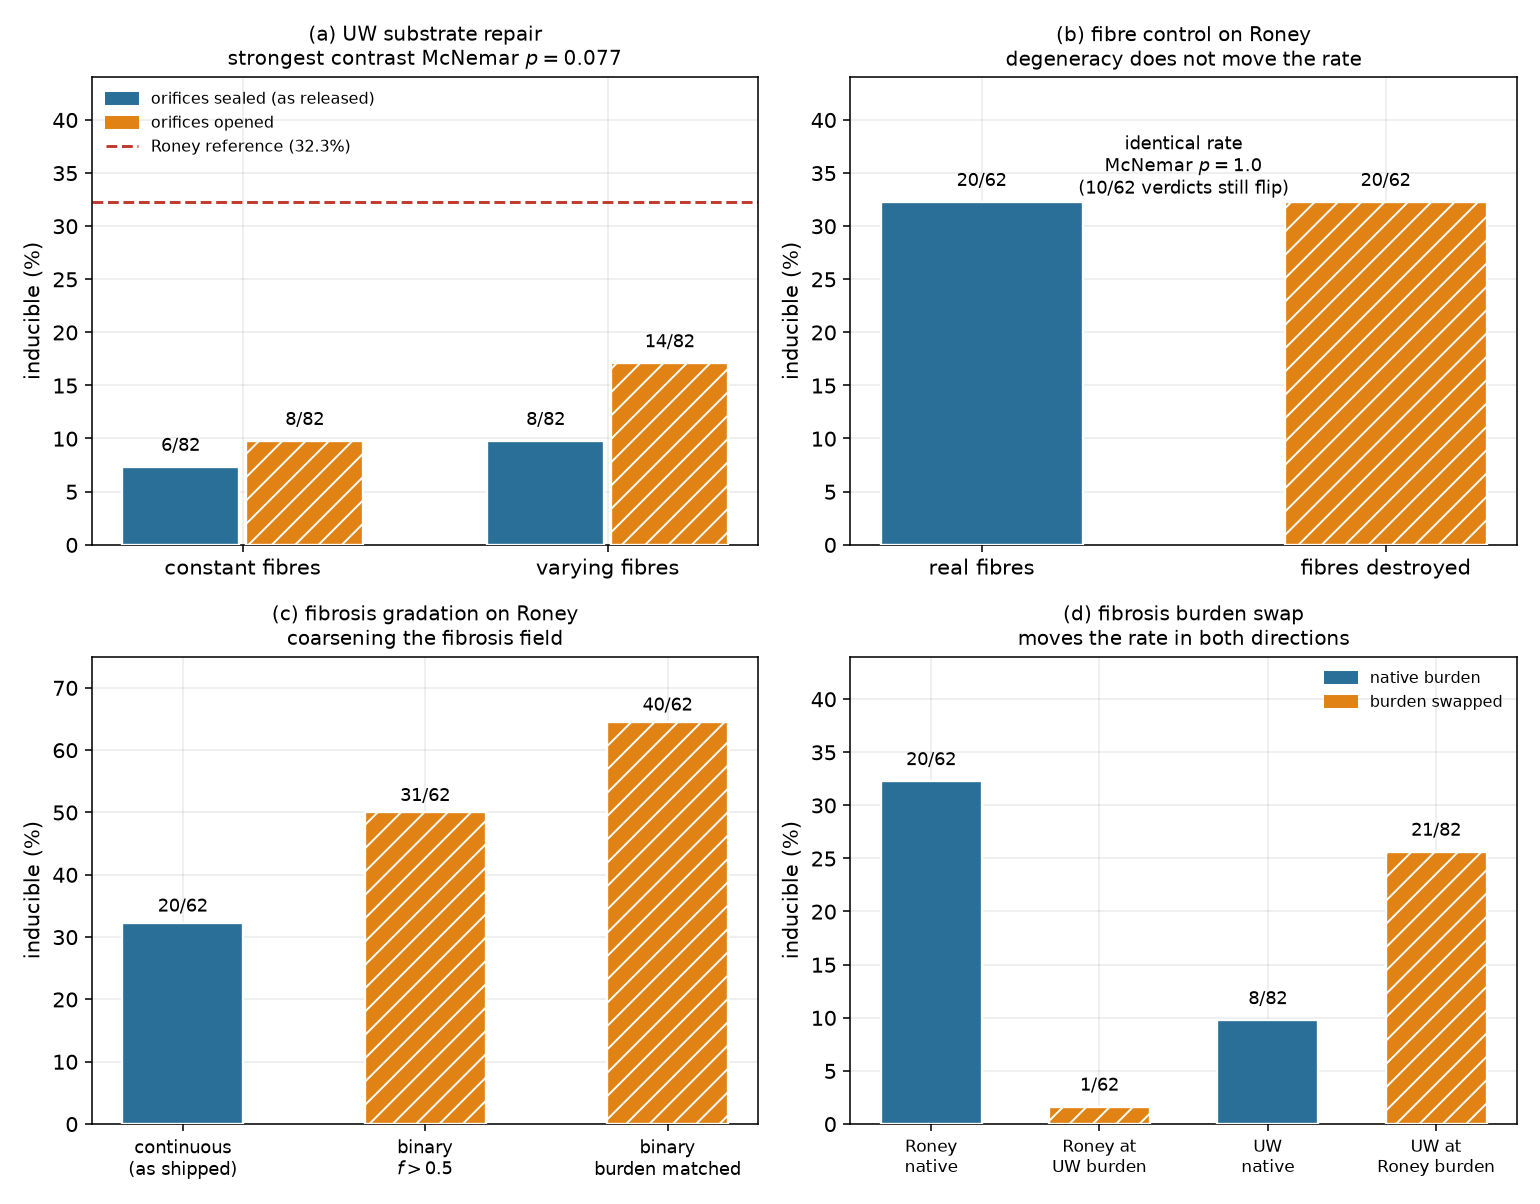
\includegraphics[width=\linewidth]{fig_substrate_audit.png}
\caption{Three controls on the substrate. (a) Repairing both UW defects raises
inducibility but not significantly, and not to the reference level. (b)
Destroying the fibre field on a cohort that has one leaves the rate exactly
unchanged. (c) Destroying the fibrosis gradation while holding mean burden fixed
roughly doubles the rate, the opposite of the predicted direction. The dashed
line is the Roney reference, $32.3\%$.}
\label{fig:substrate}
\end{figure}

Taken together the three controls leave the anomaly unexplained, and they
tighten rather than loosen the puzzle: of the two substrate defects we can
manipulate, one has no effect on the rate and the other, when imposed
deliberately, pushes it upward. Whatever suppresses reentry in the UW cohort is
not on this list. We report that as an open problem rather than close it with
the most available story, which is how the original $7\%$ came to be filed as a
cohort property in the first place.

\subsection{The labeller is reproducible in aggregate and unstable per subject}
\label{sec:labelnoise}

The controls expose something about the ground truth that matters more than the
substrate defects do. Destroying the Roney fibre field holds the aggregate rate
at exactly $20/62$ while flipping $10/62$ individual verdicts. Repairing the UW
substrate retains only two of its six original positives. The six-tier
convergence study reported below finds only $7/24$ subjects consistent across
resolutions. The aggregate inducibility rate is therefore a stable quantity, and
the per-subject verdict is not.

This is a statement about the endpoint, not an aside. The pre-registered
comparison is scored on per-subject labels, and non-differential noise in a
binary outcome attenuates any incremental AUC toward zero. Part of the null we
report is thus a property of the labeller rather than of the biomarker, and we
cannot cleanly separate the two with the present ground truth. It also sets a
floor on what any feature could achieve here, which is a limit on the whole
class of studies that score spectral or structural features against a
phenomenological inducibility verdict, not on SFI alone. The pre-registered
openCARP ground truth, substituted here for a monodomain Mitchell--Schaeffer
solver, would need to be run before the residual is attributable.

\subsection{The validity radius: why the single-vector estimator fails}
The relative error of the first-order SFI scales as $\Theta(\rhoval)$ and crosses
$10\%$ at $\rhoval^\ast\approx3$; real atria sit at median $\rhoval\approx2422$.
This proves the single-vector estimator is numerically invalid on real tissue
and $\phii_2$ is ill-conditioned, but (as boxed in Section~\ref{sec:validity})
it does not by itself prove non-predictiveness; the feature-redundancy null of
Section~\ref{sec:null} is the separate, label-dependent reason.

\subsection{The \texorpdfstring{$\rhoval$}{rho} scaling law}
\label{sec:scaling}
The gap collapses with system size by Weyl's law~\cite{weyl1912}: for a
$d$-dimensional domain the low Laplacian eigenvalues scale as $\lam_k\sim(k/N)^{2/d}$,
so $\rhoval$ grows lawfully with resolution.

\begin{table}[H]
\centering
\caption{Fitted gap-scaling exponents (gap vs.\ $N$ at fixed mean degree,
\code{results/\allowbreak rho\_scaling.json}, five-point fits).}
\label{tab:scaling}
\small
\begin{tabularx}{\linewidth}{@{}l l X@{}}
\toprule
medium & fitted gap exponent & reference \\
\midrule
real atrial surface (2-manifold) & $N^{-1.05}$ & Weyl 2-manifold $-1.0$ (within $5\%$) \\
2-D random-geometric & $N^{-1.81}$ & faster than naive $2/d$ \\
3-D random-geometric & $N^{-0.84}$ & faster than naive $2/d$ (non-monotone series) \\
\bottomrule
\end{tabularx}
\end{table}

\begin{figure}[H]
\centering
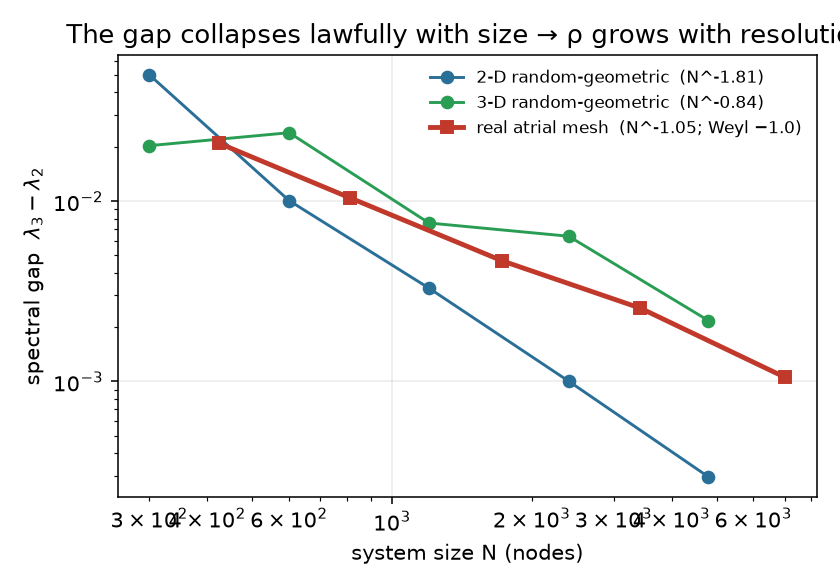
\includegraphics[width=0.82\linewidth]{fig_rho_scaling.png}
\caption{The gap collapses with mesh resolution, so the estimator degrades
\emph{more}, predictably, as the medium is meshed finer, the opposite of
``more resolution helps.'' Only the real atrial 2-manifold cleanly matches the
Weyl exponent ($-1.05$ vs.\ $-1.0$); the random-geometric exponents are reported
as ``at least as fast as Weyl,'' not law confirmations, and use the unweighted
combinatorial Laplacian.}
\label{fig:scaling}
\end{figure}

\subsection{Localization transfers across three media (weakly)}
\label{sec:localize}
The \emph{strict} pre-registered localization endpoint is null for every field,
including $\lvert\nabla\phii_2\rvert$ (median argmax-geodesic error $0.472$ is
\emph{not} below the spatial-null 5th percentile $0.406$). What survives is
weaker: $\lvert\nabla\phii_2\rvert$ is a \emph{rank} localizer (the true origin
sits in its top $\sim\!18\%$) that beats graph-centrality baselines (Perron,
weighted degree, deleted by measured correlation) and holds across media.

\begin{table}[H]
\centering
\caption{Fiedler-gradient origin-rank localization across dynamical media
(\code{results/\allowbreak gm4\allowbreak\_*\allowbreak\_metrics.json}). Lower rank is better; a perfect localizer
would place the origin at rank $0$.}
\label{tab:localize}
\small
\begin{tabularx}{\linewidth}{@{}l c c c X@{}}
\toprule
medium & $\lvert\nabla\phii_2\rvert$ origin-rank & perm-$p$ & fibrosis rank & $n$ origins \\
\midrule
FHN networks (100k)      & 0.176 & $<10^{-5}$ & $\sim0.10$ & 36{,}540 \\
Kuramoto oscillators (500) & 0.091 & $<10^{-4}$ & 0.147 & 243 \\
cardiac monodomain       & $\sim0.28$ & $<10^{-3}$ & (co-localizes) & only $\sim\!20$ \\
\bottomrule
\end{tabularx}
\end{table}

\begin{figure}[H]
\centering
\begin{subfigure}{0.49\linewidth}
  \centering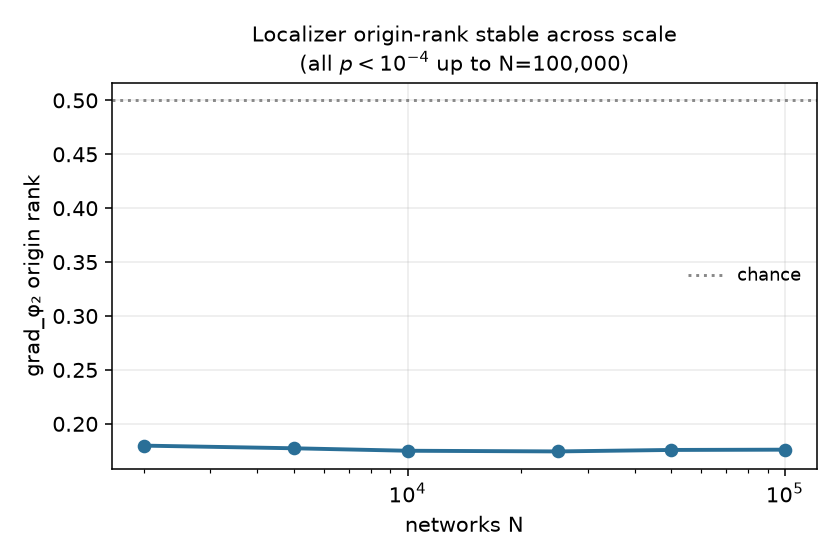
\includegraphics[width=\linewidth]{fig_localizer_ladder.png}
  \caption{origin-rank vs.\ scale}
\end{subfigure}\hfill
\begin{subfigure}{0.49\linewidth}
  \centering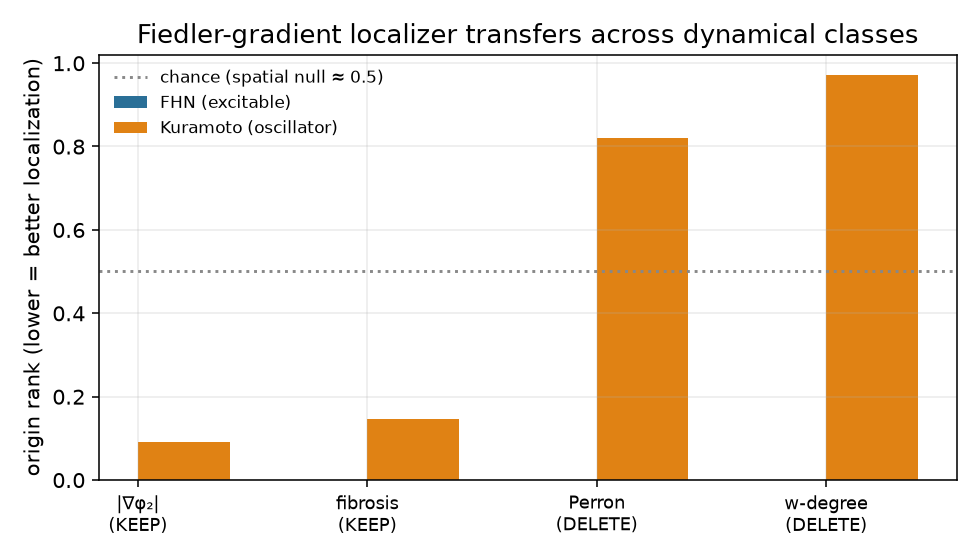
\includegraphics[width=\linewidth]{fig_localizer_transfer.png}
  \caption{transfer across media}
\end{subfigure}
\caption{The weak-rank localization pattern replicates across excitable
\emph{and} oscillator dynamics. Three caveats apply: (i)~the strict endpoint is
null, so $\lvert\nabla\phii_2\rvert$ is \emph{not} a precise localizer; (ii)~the
substrate field co-localizes, and a controlled dissociation experiment shows
why (in a diffusively-coupled medium the Fiedler bottleneck \emph{is} the
low-conduction lesion), so $\lvert\nabla\phii_2\rvert$ matches, and does not
beat, substrate imaging; (iii)~the cardiac arm rests on only $\sim\!20$ origins.}
\label{fig:localize}
\end{figure}

\subsection{The falsification protocol: what caught the false positive}
\label{sec:falsify}
Each guard, removed, manufactures a specific false positive
(\code{results/\allowbreak falsification\_\allowbreak protocol.json}). Shape-family leakage inflates AUC
by $+0.117$ (naive random-CV $0.756$ vs.\ grouped $0.640$ on a
controlled replicated cohort); the effect-size gate catches the $p$-value
trap (subspace-SFI $p\approx2\times10^{-24}$ at $N=55{,}000$, yet
$\dAUC=+0.003$ needs $\sim\!4{,}150$ cases to detect: statistically
significant, practically useless).

\begin{figure}[H]
\centering
\begin{subfigure}{0.49\linewidth}
  \centering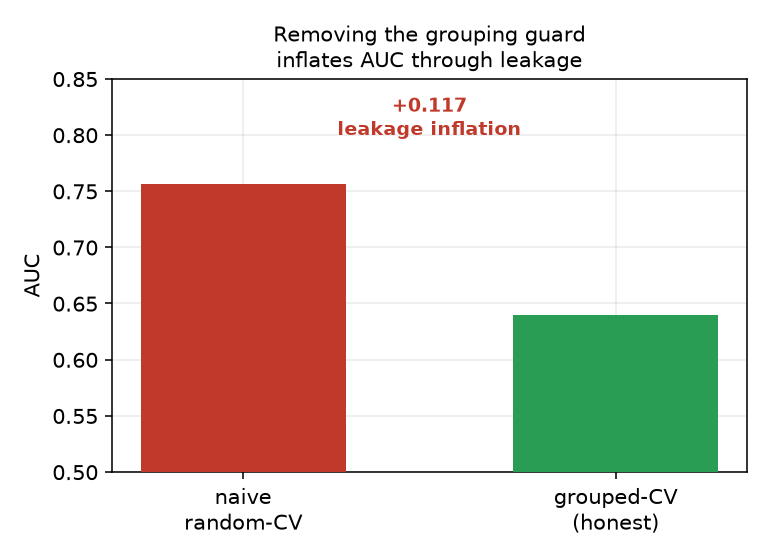
\includegraphics[width=\linewidth]{fig_falsification.png}
  \caption{leakage guard}
\end{subfigure}\hfill
\begin{subfigure}{0.49\linewidth}
  \centering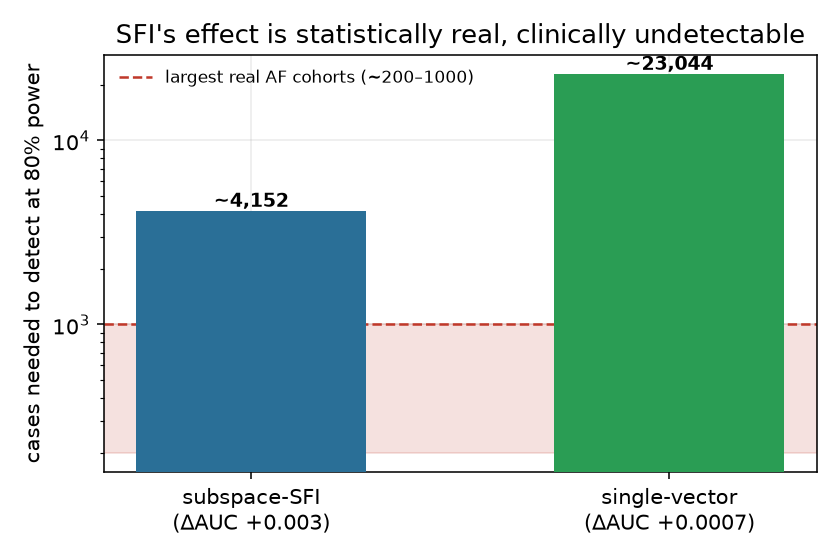
\includegraphics[width=\linewidth]{fig_power.png}
  \caption{effect-size / power gate}
\end{subfigure}
\caption{A naive analyst (random CV, $p<0.05$, no effect-size gate, no spatial
null) would have reported SFI as a working reentry biomarker. The pre-registered
protocol correctly rejects it.}
\label{fig:falsify}
\end{figure}

\subsection{Uncertainty quantification}
Morris elementary-effects screening (\code{results/e6\_metrics.json}) finds the
label most sensitive to diffusion $d_0$ ($\mu^\ast=500.7$), then fibrosis density
($147.8$) and transverse conductivity ($146.3$). A Gaussian-process surrogate has
leave-one-out $R^2=0.35$ (large residual anatomical/label variance beyond the
screened knobs, a label-noise caveat, not a positive). The synthetic null is
robust across uncoupling strengths $\Delta w\in\{0.18,0.36,0.54\}$ (grouped GBT
$\dAUC=0.033$--$0.036$, all $p\geq0.26$).

\subsection{External inducibility-rate anchor (plausibility, not validation)}
Clinically observed AF inducibility spans $\sim\!5\%$ to $\sim\!85\%$ depending on
population, protocol aggressiveness, and the sustained-AF definition (Kumar et
al.\ 2012~\cite{kumar2012} report burst-sustained $14.8\%$ vs.\
decremental-sustained $41.2\%$ \emph{in the same patients}). Our labeller's Roney
$\sim\!20$--$32\%$ sits in the moderate-burst band (Marquardt et al.\
2018~\cite{marquardt2018} report $30.6\%$ in patients without prior AF), between
the no-AF-control floor ($5\%$, Oral et al.\ 2008~\cite{oral2008}) and the
AF/aggressive ceiling ($51\%$, Kawai et al.\ 2019~\cite{kawai2019}), consistent
with $\sim\!42\%$ post-ablation (Liu et al.\ 2020~\cite{liu2020}). The UW
$\sim\!7\%$ is at/below the control floor for a cohort that \emph{is} AF patients.
We flag it as anomalous and attribute it to the substrate rather than to biology.
Two substrate defects are documented in the Limitations, and repairing both lifts
the rate to $17.1\%$ --- more than double, though still short of the $32.3\%$ seen
on fibre-carrying anatomy, so the anomaly is only partly accounted for and the
in-silico inducer may also be under-aggressive. This is a base-rate
\emph{plausibility check, not clinical validation}.

\subsection{Resolution convergence: the labeller does not converge in the tested window}
\label{sec:convergence}
Our own convergence study is the project's single weakest point, and we state it
before a reader finds it. On a completed six-tier study (Roney, $n=24$ at each of
1500/\allowbreak 3000/\allowbreak 6000/\allowbreak 12000/\allowbreak 24000/\allowbreak 48000 nodes; $144$ simulations,
\code{results/\allowbreak convergence\_summary\_roney.json}), the inducibility rate crashes
from the coarse mesh ($58.3\%$ at $1500$) to $16.7\%$ at $3000$, then is
\emph{non-monotone} across the fine tiers ($25.0\%$, $20.8\%$, $25.0\%$) and rises
again to $37.5\%$ at the finest affordable tier ($\sim\!50$k nodes), a
$17$-percentage-point spread over the last three tiers, so it has \emph{not}
settled.

\begin{table}[H]
\centering
\caption{Inducibility rate vs.\ mesh resolution (Roney, $n=24$ per tier). The
rate does not converge in the tested window; adjacent-tier per-subject verdict
agreement climbs but the rate keeps drifting.}
\label{tab:convergence}
\small
\begin{tabular}{@{}lcccccc@{}}
\toprule
nodes & 1{,}500 & 3{,}000 & 6{,}000 & 12{,}000 & 24{,}000 & 48{,}000 \\
\midrule
inducibility rate & 58.3\% & 16.7\% & 25.0\% & 20.8\% & 25.0\% & \textbf{37.5\%} \\
adj.-tier agreement & --- & 50\% & 75\% & 71\% & 62\% & 79\% \\
\bottomrule
\end{tabular}
\end{table}

\begin{figure}[H]
\centering
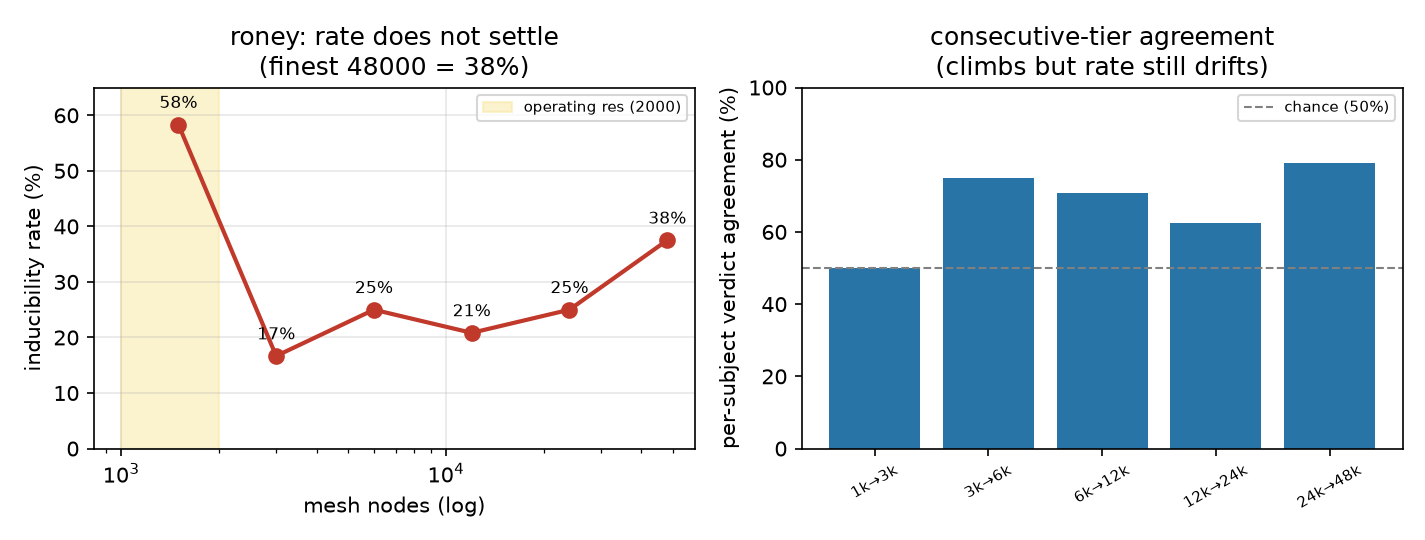
\includegraphics[width=0.9\linewidth]{fig_convergence.png}
\caption{Left: the inducibility rate does not settle; the finest tier
($48{,}000$ nodes $=37.5\%$) sits above the mid tiers. Right: adjacent-tier
per-subject verdict agreement climbs ($50\%\to79\%$) while the aggregate rate
still drifts. Only $7/24$ subjects are fully consistent across all six tiers.}
\label{fig:convergence}
\end{figure}

The convergence finding limits the absolute numbers but not the comparative
claims. The rate does \emph{not}
collapse to zero; the phenomenon is real; it is the \emph{magnitude} that is
resolution-sensitive up to $\sim\!50$k nodes. Because the main results ran at
$2{,}000$ nodes, every \emph{absolute} number (inducibility rate, competitor AUC,
localizer origins) is coarse-mesh-provisional pending the deferred openCARP
validation. What this does \emph{not} touch is what we lead with: (a)~the
\emph{relative} SFI-vs-competitor comparison, since both arms score the
\emph{same} labels, so this bias cancels; and (b)~the label-free
estimator-validity argument ($\rhoval$ is computed from the graph Laplacian, no
labels at all).

%======================================================================
\section{Discussion}
%======================================================================
This work makes four contributions.
(1)~A pre-registered, leakage-controlled, effect-size-gated evaluation of a
plausible spectral biomarker: a clean null at synthetic scale ($10^5$ networks)
with its mechanism (feature redundancy: even the exact $\Delta\lam_2$ SFI adds
nothing), and an inconclusive, underpowered verdict on real anatomy.
(2)~A label-free validity criterion $\rhoval$ for the single-vector estimator:
it proves $\phii_2$ is ill-conditioned on real tissue ($\rhoval\approx2422\gg
\rhoval^\ast\approx3$), a portable a priori check for any Fiedler-based marker,
with the caveat that $\rhoval$ bounds estimator accuracy, not predictive
content. (3)~A weak-but-real, purely connectivity-derived rank localizer that
equals substrate localization and beats centrality baselines across three media.
(4)~A demonstration that standard methodology manufactures the exact false
positives this protocol catches (leakage $+0.117$ AUC; the $p$-value trap).

The validity screen is
domain-general. Spectral-graph fragility markers are used for seizure-focus
localization, brain connectomics, and power-grid vulnerability. The same
precondition applies: compute $\rhoval=\lVert\Delta L\rVert/(\lam_3-\lam_2)$; if
$\rhoval\gg1$, the first-order spectral marker is outside its validity radius and
its in-sample correlations cannot be trusted.

We are equally explicit about what we do not claim. The mathematics is
classical; no new theorem.
$\rhoval$ does \emph{not} prove SFI is non-predictive, only that the
single-vector estimator is ill-conditioned; the null is separately due to feature
redundancy. The real-cohort result is \emph{not} a demonstrated null; it is
underpowered. The localizer is \emph{not} precise (strict endpoint null) and does
\emph{not} beat substrate imaging. The $\rhoval$ scaling ``law'' is a clean match
to Weyl only on the real atrial 2-manifold. Labels are a monodomain simulator,
not clinical outcomes and not openCARP.

%======================================================================
\section{Limitations}
%======================================================================
\begin{enumerate}[leftmargin=1.5em]
\item The labeller over-calls inducibility at the operating mesh
resolution and does not converge in the tested window (Section~\ref{sec:convergence}):
the rate drops from $58\%$ at $1500$ nodes to $17\%$ at $3000$, is non-monotone
across the fine tiers, and rises to $37.5\%$ at $\sim\!50$k nodes; only $7/24$
subjects are fully consistent across all six tiers. All \emph{absolute} rates and
AUCs are coarse-mesh-provisional; the \emph{relative} comparison scores the same
labels in both arms, so this bias cancels there.
\item Simulator, not clinical, labels: the pre-registered openCARP ground truth
was substituted with monodomain Mitchell--Schaeffer, a logged deviation.
\item The UW cohort uses a PCA-surrogate universal-atrial-coordinate map, and its
substrate carries two defects we identified only after the fact. The released
meshes have a \emph{degenerate} fibre field --- the \code{VECTORS fiber} array is
present but equals a constant $(1,0,0)$ for every element of all $164$ meshes, so
the anisotropy the solver applies is a fixed coordinate bias rather than anatomy.
Separately, we had been mapping element tag $164$ to half-fibrotic tissue when it
is in fact the set of caps over the pulmonary veins and the mitral valve. Across
all $82$ meshes it resolves into four to six large components, each a topological
disc --- five in $75$ meshes, four in five of them and six in two, which is the
usual variation in pulmonary-vein anatomy --- and it borders fibrotic elements on
only $\sim\!0.08\%$ of its incident edges against a chance expectation of
$14$--$20\%$. Removing it opens the surface, by a median of seven boundary loops.
Left in, it lets activation cross those orifices instead of circling them.
Repairing both raises inducibility from $6/82$ to $14/82$ ($7.3\%\to17.1\%$), which
does not reach paired significance (McNemar exact $p=0.077$) and closes only $39\%$
of the gap to the fibre-carrying Roney cohort ($32.3\%$). A direct control settles
the fibre half of that and overturns our first reading of it: destroying the fibre
field on the Roney cohort, which ships a real one, leaves the inducibility rate
\emph{exactly unchanged} at $20/62$ (McNemar $p=1.0$), while still perturbing the
dynamics --- sustained-reentry duration moves on $50/62$ subjects, by up to
$661$~ms. Fibre degeneracy therefore does not drive the inducibility \emph{rate},
and our initial attribution of the UW anomaly to it was wrong. The anomaly stands
unexplained. The categorical three-level fibrosis of these meshes, against Roney's
continuous $276$--$1071$-level LGE field, is the leading remaining candidate.
Either way the cohort's predictive test is uninformative about SFI.
\item The inducibility label is stable in aggregate but noisy per subject, which
attenuates every $\dAUC$ we report. Destroying the Roney fibre field holds the rate
at $20/62$ yet flips $10/62$ individual verdicts; repairing the UW substrate retains
only $2$ of its $6$ original positives. That compounds the mesh-convergence
instability above, where just $7/24$ subjects were consistent across six
resolutions. Non-differential label noise biases incremental AUC toward zero, so the
null we report is partly a statement about the labeller and not only about SFI.
\item $\sim\!30$ DeLong comparisons were run; the one positive
(\code{fibrosis\_vs\_+SFI}, $p=0.009$) is a pre-specified secondary, suggestive
not confirmatory.
\item $\rhoval^\ast$ and the random-geometric gap exponents are empirical; only
the real atrial 2-manifold cleanly matches the Weyl exponent.
\end{enumerate}

%======================================================================
\section{Conclusion}
%======================================================================
A closed-form spectral fragility index does not add practically meaningful
reentry-inducibility prediction beyond existing features at synthetic scale (a
clean, feature-redundancy null), and on real anatomy the evidence is
inconclusive rather than a demonstrated null. Independently, the single-vector
estimator is provably ill-conditioned on real tissue ($\rhoval\gg1$). The core
result is not a discovery but a carefully-scoped boundary: where a Fiedler-based
estimator is numerically valid, why real tissue lies far outside it, and how
easily naive methodology would have mistaken redundant, inconclusive signal for a
working biomarker. The absolute claims await the openCARP validation.

%======================================================================
\appendix
\section{Formal (proof-assistant) verification of the SFI algebraic core}
\label{app:formal}
%======================================================================
The algebraic core of the SFI edge-sensitivity identity is re-proved inside the
Coq 8.18 proof assistant and checked by its small trusted kernel, an assurance
level above a computer-algebra system. The primary file
(\code{formal/sfi\_edge\_identity\_Q.v}) works over the exact rationals
$\mathbb{Q}$, so \code{Print Assumptions} reports \emph{``Closed under the global
context''} for every theorem: zero axioms. A mathematically identical
companion over the reals $\mathbb{R}$ (\code{formal/sfi\_edge\_identity.v})
inherits Coq's two standard real-number-library axioms and is kept only to show
the statements hold over $\mathbb{R}$.

\begin{table}[H]
\centering
\caption{Kernel-checked theorems ($v=e_i-e_j$ the edge vector, $E_{ij}=\partial
L/\partial w_{ij}=vv^{\!\top}$). T1--T5 are axiom-free over $\mathbb{Q}$.}
\label{tab:coq}
\small
\begin{tabularx}{\linewidth}{@{}l l X@{}}
\toprule
name & statement & meaning \\
\midrule
\code{T1\_rank\_one\_quadratic\_form} & $\phii^{\!\top}(vv^{\!\top})\phii=(v\cdot\phii)^2$ & quadratic form of a rank-one edge matrix \\
\code{dot\_edge} (T2) & $(e_i-e_j)\cdot\phii=\phii_i-\phii_j$ & the edge vector selects the potential difference \\
\code{T3\_sfi\_edge\_sensitivity} & $\phii^{\!\top}E_{ij}\phii=(\phii_i-\phii_j)^2$ & \textbf{the SFI edge term} \\
\code{T4\_sfi\_term\_nonneg} & $0\leq w\Rightarrow 0\leq w(\phii_i-\phii_j)^2$ & each SFI contribution is non-negative \\
\code{T5\_aggregate\_nonneg} & $\sum(\text{nonneg terms})\geq0$ & SFI is a Dirichlet energy; the Laplacian form is PSD \\
\bottomrule
\end{tabularx}
\end{table}

Combined with the classical Hellmann--Feynman theorem
$\partial\lam_2/\partial w_{ij}=\phii_2^{\!\top}(\partial L/\partial w_{ij})\phii_2$
(Ghosh--Boyd 2006~\cite{ghosh2006}, an analysis result we cite, not re-prove),
T3 is exactly the closed form $\partial\lam_2/\partial w_{ij}=(\phii_{2,i}-\phii_{2,j})^2$.
Lean/Mathlib was attempted; its toolchain binaries are distributed only as
GitHub release assets, which the compute environment's egress policy blocks with
a hard 403, so Coq provides the equivalent kernel-checked guarantee. Reproduce
with \code{coqc formal/sfi\_edge\_identity\_Q.v}.

\section{Reproducibility}
All stochastic steps are seeded; the exact configuration and commit hash
accompany every reported number. Numeric verification:
\code{python scripts/verify\_sfi\_identity.py} and
\code{python scripts/verify\_math\_rigor.py} (sympy symbolic, mpmath 40-digit,
exact-rational, interval-certified, and cross-solver checks). Convergence:
\code{python scripts/convergence\_analyze.py roney}. Figures are regenerated by
\code{scripts/make\_paper\_figures.py}. Datasets: Roney LA cohort (Zenodo
5801337) and UW/Boyle meshes (Dryad \code{10.5061/dryad.kkwh70sg0}); both are
public and de-identified.

%======================================================================
\begin{thebibliography}{99}
%======================================================================
\bibitem{fiedler1973} M.~Fiedler. Algebraic connectivity of graphs.
\emph{Czechoslovak Mathematical Journal}, 23(2):298--305, 1973.

\bibitem{ghosh2006} A.~Ghosh and S.~Boyd. Growing well-connected graphs. In
\emph{Proc.\ 45th IEEE Conference on Decision and Control (CDC)}, 6605--6611, 2006.

\bibitem{pecora1998} L.~M.~Pecora and T.~L.~Carroll. Master stability functions
for synchronized coupled systems. \emph{Physical Review Letters}, 80(10):2109--2112, 1998.

\bibitem{barahona2002} M.~Barahona and L.~M.~Pecora. Synchronization in
small-world systems. \emph{Physical Review Letters}, 89(5):054101, 2002.

\bibitem{bomela2020} W.~Bomela, S.~Wang, C.-A.~Chou, and J.-S.~Li. Real-time
inference and detection of disruptive EEG networks for epileptic seizures.
\emph{Scientific Reports}, 10:8653, 2020.

\bibitem{weyl1912} H.~Weyl. Das asymptotische Verteilungsgesetz der Eigenwerte
linearer partieller Differentialgleichungen. \emph{Mathematische Annalen},
71(4):441--479, 1912.

\bibitem{daviskahan1970} C.~Davis and W.~M.~Kahan. The rotation of eigenvectors
by a perturbation.\ III. \emph{SIAM Journal on Numerical Analysis}, 7(1):1--46, 1970.

\bibitem{delong1988} E.~R.~DeLong, D.~M.~DeLong, and D.~L.~Clarke-Pearson.
Comparing the areas under two or more correlated receiver operating
characteristic curves: a nonparametric approach. \emph{Biometrics},
44(3):837--845, 1988.

\bibitem{sunxu2014} X.~Sun and W.~Xu. Fast implementation of DeLong's algorithm
for comparing the areas under correlated ROC curves. \emph{IEEE Signal
Processing Letters}, 21(11):1389--1393, 2014.

\bibitem{mitchell2003} C.~C.~Mitchell and D.~G.~Schaeffer. A two-current model
for the dynamics of cardiac membrane. \emph{Bulletin of Mathematical Biology},
65(5):767--793, 2003.

\bibitem{roney2022} C.~H.~Roney et al. Predicting atrial fibrillation recurrence
by combining population data and virtual cohorts of patient-specific left-atrial
models. \emph{Circulation: Arrhythmia and Electrophysiology}, 15(2):e010253, 2022.
doi:10.1161/CIRCEP.121.010253. Data: Zenodo 5801337.

\bibitem{uwboyle2025} S.~Bifulco, P.~M.~Boyle, et al. Predicting arrhythmia
recurrence post-ablation in atrial fibrillation using explainable machine
learning. \emph{Communications Medicine}, 2025.
doi:10.1038/s43856-025-01058-4. Data: Dryad \code{10.5061/dryad.kkwh70sg0}.

\bibitem{khurram2014} I.~M.~Khurram et al. Magnetic resonance image intensity
ratio, a normalized measure to enable interpatient comparability of left atrial
fibrosis. \emph{Heart Rhythm}, 11(1):85--92, 2014.

\bibitem{kumar2012} S.~Kumar et al. Atrial fibrillation inducibility in the
absence of structural heart disease or clinical atrial fibrillation: critical
dependence on induction protocol, inducibility definition, and number of
inductions. \emph{Circulation: Arrhythmia and Electrophysiology}, 5(3):531--536,
2012. PMID 22528047.

\bibitem{marquardt2018} J.~Marquardt et al. Prognostic value of atrial
fibrillation inducibility in patients without history of clinical atrial
fibrillation. \emph{Journal of Atrial Fibrillation}, 11(1):1837, 2018.
PMID 30455834.

\bibitem{oral2008} H.~Oral et al. Inducibility of paroxysmal atrial fibrillation
by isoproterenol and its relation to the mode of onset of atrial fibrillation.
\emph{Journal of Cardiovascular Electrophysiology}, 19(5):466--470, 2008.
PMID 18266669.

\bibitem{kawai2019} S.~Kawai et al. Predictive value of the induction test with
atrial burst pacing with regard to long-term recurrence after ablation in
persistent atrial fibrillation. \emph{Journal of Arrhythmia}, 35(2):223--229,
2019. PMID 31007786.

\bibitem{liu2020} X.~Liu et al. Is atrial fibrillation noninducibility by burst
pacing after catheter ablation associated with reduced clinical recurrence? A
systematic review and meta-analysis. \emph{Journal of the American Heart
Association}, 9(14):e015260, 2020. PMID 32654581.
\end{thebibliography}

\end{document}
